\documentclass[12pt, letterpaper]{article}
\usepackage{graphicx}
\usepackage{minted}
\usepackage{xcolor}

\definecolor{monokaibg}{HTML}{272822}
\definecolor{friendlybg}{HTML}{f0f0f0}
\graphicspath{ {./images/} }

\title{Machine Learning, ICS3206, Course Project 2020}
\author{Liam Attard [0299300L]}
\date{}

\begin{document}

    \maketitle

    \section{Viola-Jones technical discussion}
        \subsection{Introduction}
            The Viola-Jones paper (Rapid Object Detection using a
            Boosted Cascade of Simple Features) describes a machine
            learning technique that achieves a fast and accurate
            object recognition method that isn’t based on deep learning.
            This report is still relevant today especially for face
            detection and has been cited around 22,000 times. The
            technique used is achieved from the following three steps:
            \begin{itemize}
                \item The image is first represented using a summed-area table
                called the integral image.
                \item The principal features of the target object are picked
                out from a training set using an algorithm based on AdaBoost
                and generates efficient classifiers.
                \item The image is then passed through several filters, 
                referred to as a "cascade structure” which is, in essence, a
                degenerate decision tree. Each filter focuses more on the
                object itself and ignores the noise.

            \end{itemize}
            This paper’s detector was tested on 384 by 288 images at 15 frames
            per second and found to be accurate irrelevant of facial features 
            and ethnicity. The prompt detection of this technique is what
            makes it ahead of other methods.

        \subsection{The Integral Image}
            \subsubsection{Haar-Like Features}
                Haar features are rectangular features maked over an image.
                To calculate these principal features of an image several 
                computations are performed. 

                \begin{figure}[h]
                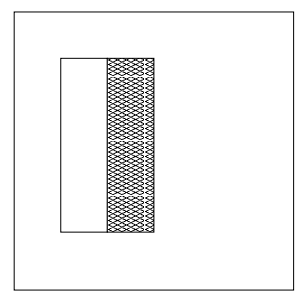
\includegraphics[scale=0.3]{sampleOne.png}
                \centering
                \caption{Shows an example of a feature where the sum of
                pixels in the white rectangle is subtracted from the sum
                of pixels in the grey rectangle. By performing these 
                calculations on raw image values, the result can take a
                lot of time so that is why calculating the integral image
                any rectangular value can be performed quickly and in
                constant time.}
                \end{figure}
                \begin{figure}[H]
                    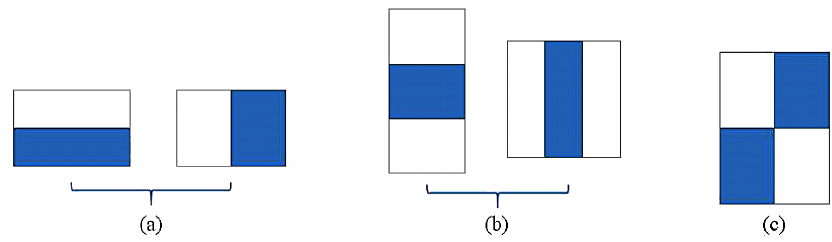
\includegraphics[scale=0.3]{features.png}
                    \centering
                    \caption{ Shows different ways of calculating the 
                    features, (a) shows two-rectangle features, (b) shows
                    three-rectangle features and (c) shows a four-rectangle
                    feature.}
                    
                \end{figure}

            \subsubsection{Calculating The Integral Image}
                The integral image is found by iterating over each pixel
                and computing its new value, which is obtained by
                calculating the sum of pixels above and to the left of it.
                The original pixel i(x,y)’s integral image ii(x,y) can be
                found by using the following equation.

                \begin{center}
                    \(ii(x,y)= \sum_{(x \leq x,y' \leq y)}\)
                \end{center}

                \begin{center}
                    \begin{tabular}{ |c|c| }
                    \hline
                    1 & 5 \\ 
                    \hline
                    2 & 4 \\  
                    \hline
                    \end{tabular}

                    Original Image
                \end{center}
                The Matrix below shows an example of an original image 
                alongside its integral image. 

                \begin{center}
                    \begin{tabular}{ |c|c| }
                    \hline
                    1 & 6 \\ 
                    \hline
                    3 & 12 \\  
                    \hline
                    \end{tabular}

                    Integral Image
                \end{center}

            \subsubsection{Integral Image PseudoCode}
            \begin{minted}[
                style=monokai,
                bgcolor=monokaibg
            ]{python}
for each pixel(x2,y2):
    for x in x1 to x2:
        for y in y1 to y2:
            sum += Arr[x][y]
            \end{minted}
            Where x1 is the row number of the top-left pixel [0,0], y1
            is the column number of the top-left pixel [0,0], x2 is the
            row number of the bottom-right pixel, y2  is the column
            number of the bottom-right pixel.

            \subsubsection{Calculating the Sum of Any Pixel Value From the Integral Image}
            Consider the following matrix:
            \begin{figure}[h]
                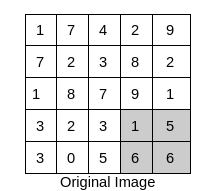
\includegraphics[scale=0.5]{photo1.png}
                \centering
            \end{figure}
            \\ The sum of the greyed out area is 1+5+6+6 which is 18. Now
            consider its integral image:
            \begin{figure}[h]
                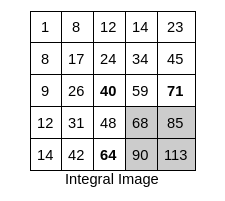
\includegraphics[scale=0.5]{photo2.png}
                \centering
            \end{figure}
            \\ To Calculate the sum of the greyed out area subtract the
            summation of the unwanted areas, in this case: 113 - 64 -
            71 which is  -22 and re-add the areas that have been taken
            off twice in this case -22+40 which is 18. Although in
            this case, it didn’t make sense to calculate the integral
            image given how small the size of the original image is,
            in pictures with a very high resolution, this would save
            a lot of time. 
    
        \subsection{Learning Classification Functions Using AdaBoost}
            Over 180,000 features can be calculated given that
            the detector is of size 24x24 pixels. This number of
            features can be in danger of both slow classification
            and overfitting. In order to avoid such problems 
            a boosting algorithm, AdaBoost, is used to select a small
            set of critical Haar-like features using weak classifiers.
            For each of the features the algorithm finds the function which separates
            them positively (contain a face) and negatively (don’t
            contain a face) in the most optimal way ie. leaving the
            least possible number of values misclassified. Given a
            24 by 24 image \(x\) with feature \(f_j\), a weak classifier \((h_j)\), is 
            defined by 
            
            \begin{center}
                \(h_j(x)=1\) if \(p_j f_j < p_j\theta_j\) \\
                \(h_j(x)=0\) otherwise
            \end{center}
            where \(\theta_j\) is the treshold and \(p_j\) indicates
            the direction of the inequality sign.
            
            \subsubsection{Resultant Features}

                For the Viola-Jones algorithm a very aggresive
                approach which selects only a few number of features
                was implemented. 


                \begin{figure}[H]
                    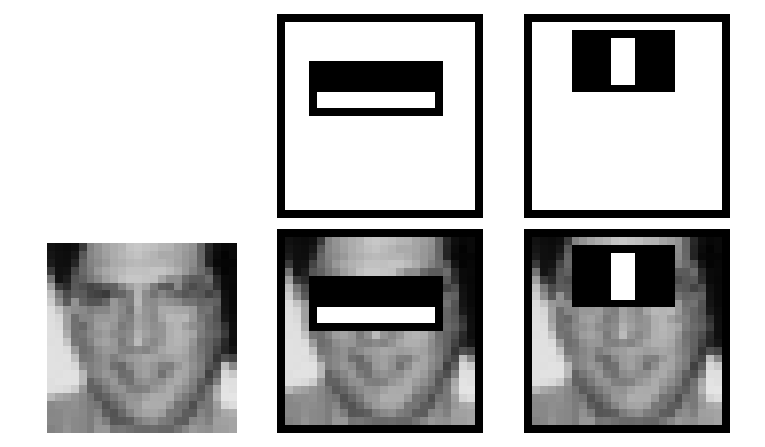
\includegraphics[scale=0.3]{selectedFeatures.png}
                    \centering
                    \caption{The figure shows how the top two features AdaBoost
                    gave priority to are the darker eye area over the
                    cheeks and the bridge of the nose.}
                \end{figure}

        \subsection{Cascade of Classifiers}
        ,

                

\end{document}

